\documentclass{standalone}
\usepackage{tikz}
\usetikzlibrary{patterns, positioning}


\begin{document}
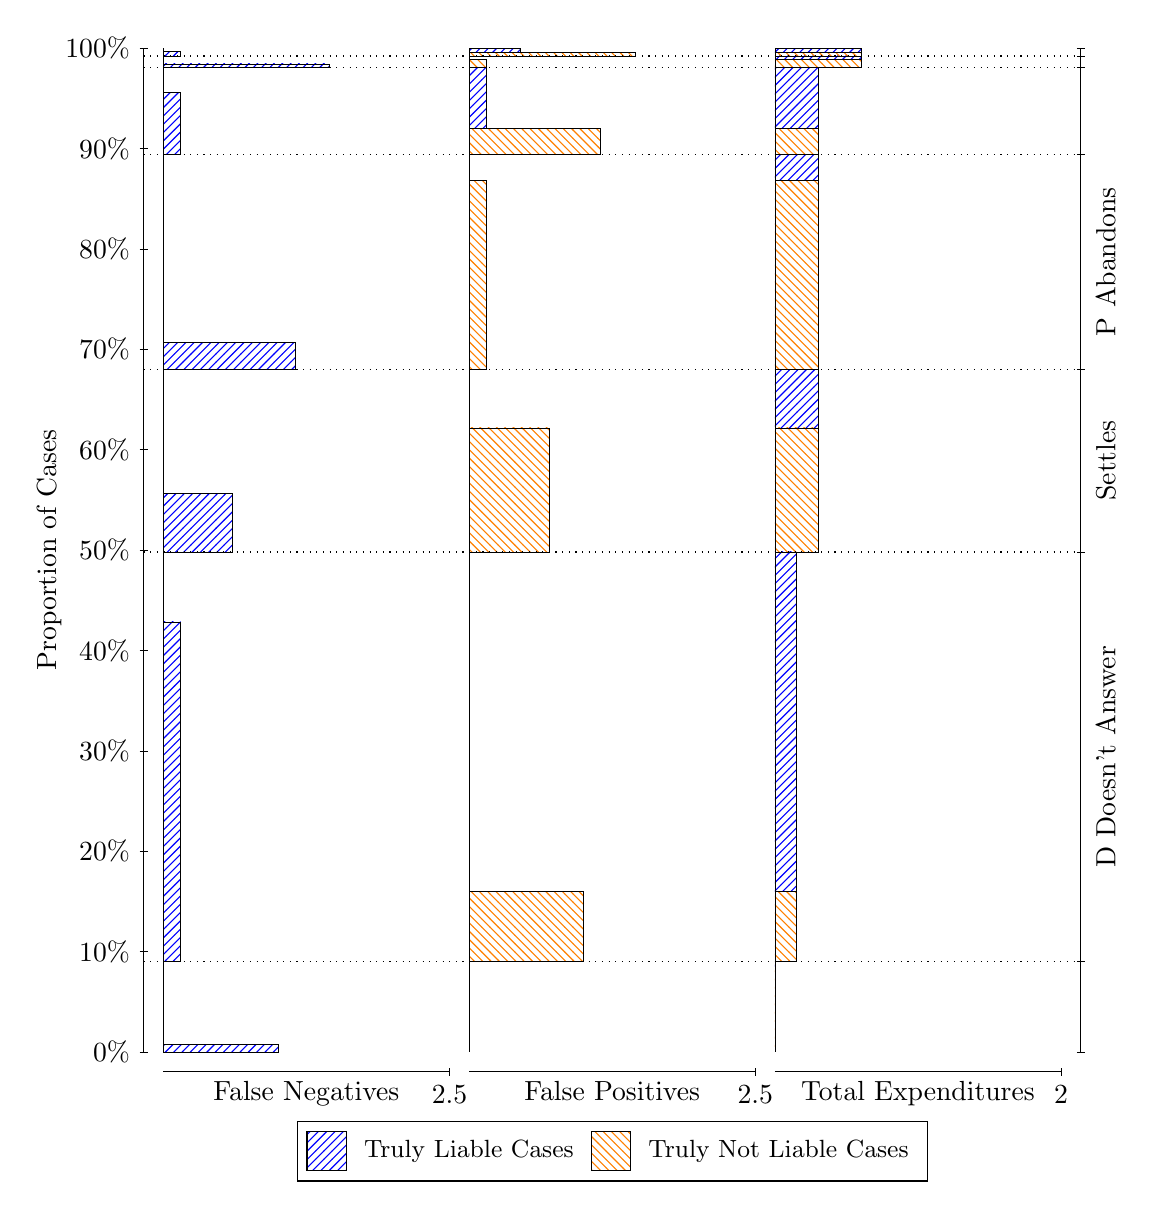
\begin{tikzpicture}
\draw[black, very thin] (1.5,1.75) -- (1.5,14.5);
\node[rotate=90, text=black, anchor=center] at (0.3, 8.125) {Proportion of Cases};
\draw[black, very thin] (1.45,1.75) -- (1.55,1.75);
\node[text=black, anchor=east] at (1.45, 1.75) {0\%};
\draw[black, very thin] (1.45,3.025) -- (1.55,3.025);
\node[text=black, anchor=east] at (1.45, 3.025) {10\%};
\draw[black, very thin] (1.45,4.3) -- (1.55,4.3);
\node[text=black, anchor=east] at (1.45, 4.3) {20\%};
\draw[black, very thin] (1.45,5.575) -- (1.55,5.575);
\node[text=black, anchor=east] at (1.45, 5.575) {30\%};
\draw[black, very thin] (1.45,6.85) -- (1.55,6.85);
\node[text=black, anchor=east] at (1.45, 6.85) {40\%};
\draw[black, very thin] (1.45,8.125) -- (1.55,8.125);
\node[text=black, anchor=east] at (1.45, 8.125) {50\%};
\draw[black, very thin] (1.45,9.4) -- (1.55,9.4);
\node[text=black, anchor=east] at (1.45, 9.4) {60\%};
\draw[black, very thin] (1.45,10.675) -- (1.55,10.675);
\node[text=black, anchor=east] at (1.45, 10.675) {70\%};
\draw[black, very thin] (1.45,11.95) -- (1.55,11.95);
\node[text=black, anchor=east] at (1.45, 11.95) {80\%};
\draw[black, very thin] (1.45,13.225) -- (1.55,13.225);
\node[text=black, anchor=east] at (1.45, 13.225) {90\%};
\draw[black, very thin] (1.45,14.5) -- (1.55,14.5);
\node[text=black, anchor=east] at (1.45, 14.5) {100\%};

\draw[black, very thin] (13.4,1.75) -- (13.4,14.5);
\draw[black, very thin] (13.35,1.75) -- (13.45,1.75);
\node[anchor=west] at (13.35, 1.75) {};
\draw[black, very thin] (13.35,2.8981) -- (13.45,2.8981);
\node[anchor=west] at (13.35, 2.8981) {};
\draw[black, very thin] (13.35,8.0999) -- (13.45,8.0999);
\node[anchor=west] at (13.35, 8.0999) {};
\draw[black, very thin] (13.35,10.423) -- (13.45,10.423);
\node[anchor=west] at (13.35, 10.423) {};
\draw[black, very thin] (13.35,13.153) -- (13.45,13.153);
\node[anchor=west] at (13.35, 13.153) {};
\draw[black, very thin] (13.35,14.256) -- (13.45,14.256);
\node[anchor=west] at (13.35, 14.256) {};
\draw[black, very thin] (13.35,14.399) -- (13.45,14.399);
\node[anchor=west] at (13.35, 14.399) {};
\draw[black, very thin] (13.35,14.5) -- (13.45,14.5);
\node[anchor=west] at (13.35, 14.5) {};

\draw[black, very thin, pattern color=blue, pattern=north east lines] (1.75,1.75) rectangle (3.2033,1.8447);
\draw[black, very thin, pattern color=orange, pattern=north west lines] (1.75,1.8447) rectangle (1.75,2.8981);
\draw[black, very thin, pattern color=blue, pattern=north east lines] (1.75,2.8981) rectangle (1.968,7.212);
\draw[black, very thin, pattern color=orange, pattern=north west lines] (1.75,7.212) rectangle (1.75,8.0999);
\draw[black, very thin, pattern color=blue, pattern=north east lines] (1.75,8.0999) rectangle (2.622,8.8464);
\draw[black, very thin, pattern color=orange, pattern=north west lines] (1.75,8.8464) rectangle (1.75,10.423);
\draw[black, very thin, pattern color=blue, pattern=north east lines] (1.75,10.423) rectangle (3.4213,10.76);
\draw[black, very thin, pattern color=orange, pattern=north west lines] (1.75,10.76) rectangle (1.75,13.153);
\draw[black, very thin, pattern color=blue, pattern=north east lines] (1.75,13.153) rectangle (1.968,13.934);
\draw[black, very thin, pattern color=orange, pattern=north west lines] (1.75,13.934) rectangle (1.75,14.256);
\draw[black, very thin, pattern color=blue, pattern=north east lines] (1.75,14.256) rectangle (3.8573,14.299);
\draw[black, very thin, pattern color=orange, pattern=north west lines] (1.75,14.299) rectangle (1.75,14.399);
\draw[black, very thin, pattern color=blue, pattern=north east lines] (1.75,14.399) rectangle (1.968,14.458);
\draw[black, very thin, pattern color=orange, pattern=north west lines] (1.75,14.458) rectangle (1.75,14.5);
\draw[black, very thin, pattern color=orange, pattern=north west lines] (5.6333,1.75) rectangle (5.6333,2.8034);
\draw[black, very thin, pattern color=blue, pattern=north east lines] (5.6333,2.8034) rectangle (5.6333,2.8981);
\draw[black, very thin, pattern color=orange, pattern=north west lines] (5.6333,2.8981) rectangle (7.0867,3.786);
\draw[black, very thin, pattern color=blue, pattern=north east lines] (5.6333,3.786) rectangle (5.6333,8.0999);
\draw[black, very thin, pattern color=orange, pattern=north west lines] (5.6333,8.0999) rectangle (6.6507,9.6767);
\draw[black, very thin, pattern color=blue, pattern=north east lines] (5.6333,9.6767) rectangle (5.6333,10.423);
\draw[black, very thin, pattern color=orange, pattern=north west lines] (5.6333,10.423) rectangle (5.8513,12.816);
\draw[black, very thin, pattern color=blue, pattern=north east lines] (5.6333,12.816) rectangle (5.6333,13.153);
\draw[black, very thin, pattern color=orange, pattern=north west lines] (5.6333,13.153) rectangle (7.3047,13.475);
\draw[black, very thin, pattern color=blue, pattern=north east lines] (5.6333,13.475) rectangle (5.8513,14.256);
\draw[black, very thin, pattern color=orange, pattern=north west lines] (5.6333,14.256) rectangle (5.8513,14.356);
\draw[black, very thin, pattern color=blue, pattern=north east lines] (5.6333,14.356) rectangle (5.6333,14.399);
\draw[black, very thin, pattern color=orange, pattern=north west lines] (5.6333,14.399) rectangle (7.7407,14.441);
\draw[black, very thin, pattern color=blue, pattern=north east lines] (5.6333,14.441) rectangle (6.2873,14.5);
\draw[black, very thin, pattern color=orange, pattern=north west lines] (9.5167,1.75) rectangle (9.5167,2.8034);
\draw[black, very thin, pattern color=blue, pattern=north east lines] (9.5167,2.8034) rectangle (9.5167,2.8981);
\draw[black, very thin, pattern color=orange, pattern=north west lines] (9.5167,2.8981) rectangle (9.7892,3.786);
\draw[black, very thin, pattern color=blue, pattern=north east lines] (9.5167,3.786) rectangle (9.7892,8.0999);
\draw[black, very thin, pattern color=orange, pattern=north west lines] (9.5167,8.0999) rectangle (10.062,9.6767);
\draw[black, very thin, pattern color=blue, pattern=north east lines] (9.5167,9.6767) rectangle (10.062,10.423);
\draw[black, very thin, pattern color=orange, pattern=north west lines] (9.5167,10.423) rectangle (10.062,12.816);
\draw[black, very thin, pattern color=blue, pattern=north east lines] (9.5167,12.816) rectangle (10.062,13.153);
\draw[black, very thin, pattern color=orange, pattern=north west lines] (9.5167,13.153) rectangle (10.062,13.475);
\draw[black, very thin, pattern color=blue, pattern=north east lines] (9.5167,13.475) rectangle (10.062,14.256);
\draw[black, very thin, pattern color=orange, pattern=north west lines] (9.5167,14.256) rectangle (10.607,14.356);
\draw[black, very thin, pattern color=blue, pattern=north east lines] (9.5167,14.356) rectangle (10.607,14.399);
\draw[black, very thin, pattern color=orange, pattern=north west lines] (9.5167,14.399) rectangle (10.607,14.441);
\draw[black, very thin, pattern color=blue, pattern=north east lines] (9.5167,14.441) rectangle (10.607,14.5);
\draw[black, dotted] (1.5,2.8981) -- (13.4,2.8981);
\draw[black, dotted] (1.5,8.0999) -- (13.4,8.0999);
\draw[black, dotted] (1.5,10.423) -- (13.4,10.423);
\draw[black, dotted] (1.5,13.153) -- (13.4,13.153);
\draw[black, dotted] (1.5,14.256) -- (13.4,14.256);
\draw[black, dotted] (1.5,14.399) -- (13.4,14.399);
\draw[black, very thin] (1.75,1.5) -- (5.3833,1.5);
\node[text=black, anchor=north] at (3.5667, 1.5) {False Negatives};
\draw[black, very thin] (5.3833,1.45) -- (5.3833,1.55);
\node[text=black, anchor=north] at (5.3833, 1.45) {2.5};

\draw[black, very thin] (5.6333,1.5) -- (9.2667,1.5);
\node[text=black, anchor=north] at (7.45, 1.5) {False Positives};
\draw[black, very thin] (9.2667,1.45) -- (9.2667,1.55);
\node[text=black, anchor=north] at (9.2667, 1.45) {2.5};

\draw[black, very thin] (9.5167,1.5) -- (13.15,1.5);
\node[text=black, anchor=north] at (11.333, 1.5) {Total Expenditures};
\draw[black, very thin] (13.15,1.45) -- (13.15,1.55);
\node[text=black, anchor=north] at (13.15, 1.45) {2};


\node[text=black, centered, rotate=90] at (13.72, 5.499) {D Doesn't Answer};
\node[text=black, centered, rotate=90] at (13.72, 9.2615) {Settles};
\node[text=black, centered, rotate=90] at (13.72, 11.788) {P Abandons};




\draw (7.449999999999999,1.5) node[draw=none] (baseCoordinate) {};
\begin{scope}[align=center]
        \matrix[scale=0.5, draw=black, below=0.5cm of baseCoordinate, nodes={draw}, column sep=0.1cm]{
            \node[rectangle, draw, minimum width=0.5cm, minimum height=0.5cm, pattern color=blue, pattern=north east lines] {}; &
            \node[draw=none, font=\small, text=black] (B) {Truly Liable Cases}; &
            \node[rectangle, draw, minimum width=0.5cm, minimum height=0.5cm, pattern color=orange, pattern=north west lines] {}; &
            \node[draw=none, font=\small, text=black] (B) {Truly Not Liable Cases}; \\
            };
\end{scope}

\end{tikzpicture}
\end{document}